% !TeX program = xelatex
\documentclass[withoutpreface,bwprint]{cumcmthesis}
\graphicspath{{../../../outputs/figures/}{../../../outputs/question2_analysis/}{../../../outputs/question4_analysis/}}
\title{多源公开数据约束下秦皇岛旅游客流预测与资源协同配置}
\tihao{B}
\baominghao{}
\schoolname{}
\membera{}
\memberb{}
\memberc{}
\supervisor{}
\yearinput{2026}
\monthinput{08}
\dayinput{11}
\newcommand{\paperTableWidth}{0.86\textwidth}

\begin{document}
\maketitle

\begin{abstract}
针对秦皇岛全市及北戴河、海港--阿那亚、山海关三片区在日级真实客流、停车占用和接驳调度台账不完整条件下的旅游管理问题，本文构建``客流尺度统一--预测--资源配置--情景重优化''的四阶段方法。首先，以官方年度国内游客量为绝对尺度，以景区排行观测、日历、天气和搜索主题构建三区连续日级相对旅游压力；对未上榜景点采用左删失处理，避免将未展示误作零客流。其次，采用年度增长预测与片区动态 Ridge 预测相结合的方法，输出 2026 年全市年度规模和三区日级分位情景，并以片区 split-conformal 校准报告不确定性。再次，将游客规模换算为停车泊位需求、接驳车辆需求和三班制人员需求，在停车容量、服务班距与班次覆盖约束下搜索离散资源方案。最后，对大型活动和连续降雨情景实施重优化。结果表明：2026 年全市点预测为 9,971.43 万人次；北戴河、海港--阿那亚和山海关暑期日峰值的中位情景分别为 12.75 万、5.82 万和 13.55 万人次。高压情景下，停车缺口应转化为外圈 P+R、预约与错峰需求，而非虚构新增供给。全文将日级客流、资源规模和成本均明确标注为锚点约束估计或情景规划量，不将其表述为运营实测台账。

\keywords{旅游客流\quad 尺度约束\quad 日级预测\quad 资源配置\quad 情景优化}
\end{abstract}

\section{问题重述}
秦皇岛旅游活动具有显著暑期性、节假日脉冲和片区异质性。题目要求构建游客时序、预测未来客流、制定停车--接驳--人员配置，并评估突发场景。困难在于公开数据的统计口径并不一致：全市年度数据具有绝对量，片区日级数据多为景区排行指数或报道锚点，停车和接驳数据也多为设施节点或计划班距。

因此，本文不将缺失记录补造为实测值，而将问题拆为四层：Q1 用年度总量约束日级压力形态；Q2 输出年度点预测与片区日级分位情景；Q3 将需求情景换算为独立量纲的泊位、车辆和人员；Q4 在活动、降雨扰动下重新优化。该路线保证每一层的输出均可追溯至上一层的口径。

\section{问题分析}
四个问题具有由“量”到“策”的递进关系。问题一先解决公开数据粒度不统一的问题，给出受年度总量约束的日级形态；问题二在此基础上比较预测基准并给出未来客流情景；问题三将预测情景转换为泊位、接驳车辆和班次人员的协同需求；问题四考察活动与降雨冲击下的资源重配置。各问均将缺失运营台账显式保留为参数或不确定性边界。

\section{模型假设与符号说明}
\subsection{符号说明与数据口径}
表\ref{tab:data}给出进入主线的数据层级。搜索量仅作需求代理变量，天气词不进入旅游需求主题；不匹配三区范围的景区报道只作合理性核验，不计入误差。

\begin{table}[H]\centering\small
\renewcommand{\arraystretch}{1.15}\setlength{\tabcolsep}{4pt}
\caption{主线数据及使用口径}\label{tab:data}
\begin{tabular*}{\paperTableWidth}{@{\extracolsep{\fill}}p{2.8cm}p{1.6cm}p{2.0cm}p{4.0cm}@{}}\toprule
数据层 & 时间跨度 & 粒度 & 主线用途\\ \midrule
全市国内游客量 & 2002--2024 & 年度 & 绝对尺度锚点与年度预测\\
景区排行、天气、节假日、搜索主题 & 2023--2025（搜索扩展至2016--2026） & 日级 & 三区相对压力与日级协变量\\
公开客流报道锚点 & 2023--2025 & 节假日/暑期 & 尺度校准或外部合理性核验\\
停车、接驳公开锚点 & 2014--2026 & 节点/班距 & Q3 容量边界和服务班距参照\\ \bottomrule
\end{tabular*}
\end{table}

设 $Y_y$ 为第 $y$ 年全市官方年度国内游客量，$F_{r,t}$ 为片区 $r$ 在日期 $t$ 的相对旅游压力，$V_{r,t}^{(q)}$ 为锚点约束下的日级游客规模情景，$P_t,N_t,S_t$ 分别为泊位、接驳车辆与三班制人员需求。除 $Y_y$ 外，本文不将上述量称为逐日实测统计。

\subsection{基本假设}
公开锚点在地域和统计范围一致时可校准尺度；服务班距可作为服务水平约束，但不能反推实际车辆数或载客量；未公布泊位数的停车场只作为换乘节点；车辆座位、满载率、私家车出行比例和服务效率均作为显式情景参数。

\section{模型建立与求解}
\subsection{数据预处理与四问衔接}
为避免不同统计口径在模型中被混用，先按“数据层--可用范围--用途”完成预处理：年度官方游客量仅保留为全市绝对尺度；三区 2023--2025 年片区--日期记录按日期去重并统一日历、天气和搜索的日期键；景区榜单未出现的记录保留为低于展示阈值的左删失信息，不以零客流填补；外部报道仅在地域、时间与统计范围同时匹配时参与锚点校准，其余仅作合理性核验。由此得到 23 条年度锚点和 3,288 条片区--日期记录（每片区 1,096 条）。停车、接驳报道只提取为容量边界或服务水平参照，不反推未公开的实际运营台账。

四问之间按同一口径递进：Q1 生成年度总量约束下的日级形态，Q2 将其外推为 2026 年分位情景，Q3 将每个情景换算为资源需求并求可行配置，Q4 只更新受扰动日期的需求参数后沿用 Q3 的目标和约束重优化。因此，后一问不会重新定义前一问的游客规模。
\begin{figure}[H]\centering
\setlength{\fboxsep}{7pt}
\fbox{\parbox{0.82\textwidth}{\centering
\textbf{年度官方总量与日级相对压力}\quad$\Longrightarrow$\quad
\textbf{2026 年分位客流情景}\\[-1pt]
$\Longrightarrow$\quad\textbf{泊位--接驳--人员配置}\quad$\Longrightarrow$\quad
\textbf{活动/降雨下的重优化}\\[-1pt]
\small Q1：尺度统一 \quad Q2：预测与区间 \quad Q3：资源决策 \quad Q4：扰动更新}}
\caption{四问的数据流、模型流与决策流}\label{fig:workflow}
\end{figure}

\subsection{问题一：多尺度客流时序构建}
\subsubsection{相对压力层与年度尺度层}
对片区压力取对数变换 $z_{r,t}=\log(1+F_{r,t})$，构建
\begin{equation}
z_{r,t}=a_r+\phi_rz_{r,t-1}+\boldsymbol\beta^{\mathsf T}\mathbf X_t+\delta_{r,S_t}+\varepsilon_{r,t},
\end{equation}
其中 $\mathbf X_t$ 包含滞后搜索、周末、法定假日和天气，$S_t$ 表示常态、暑期和节假日冲击状态。模型用于区分可解释短期因素与剩余波动，不作因果解释。将三区压力形态归一化为年度日权重，得到
\begin{equation}
w_t=\frac{\sum_r\exp(z_{r,t})}{\sum_{\tau\in y}\sum_r\exp(z_{r,\tau})},\qquad \widehat Y_t=Y_yw_t,
\end{equation}
从而严格满足 $\sum_{t\in y}\widehat Y_t=Y_y$。

\subsubsection{结果与解释}
2023 年和 2024 年全市官方国内游客量分别为 80,255.2 千人次和 89,457.2 千人次\cite{qhdstat}。图\ref{fig:q1annual}反映长期恢复趋势；图\ref{fig:q1pressure}用于识别三区的时季高压窗口，而非比较三区真实人数大小。未上榜景点被保留为左删失信息，避免零值偏差。

尺度校准包含两项可复核检查：其一，式(2)使每个年度的日级估计之和等于该年度官方总量，故不会偏离绝对尺度；其二，片区序列只承担相对形态识别，范围不一致的景区报道不纳入误差计算。该处理将“绝对量是否可信”和“日级形态是否合理”分开检验，避免用少量报道锚点伪造连续实测客流。

\begin{figure}[H]\centering
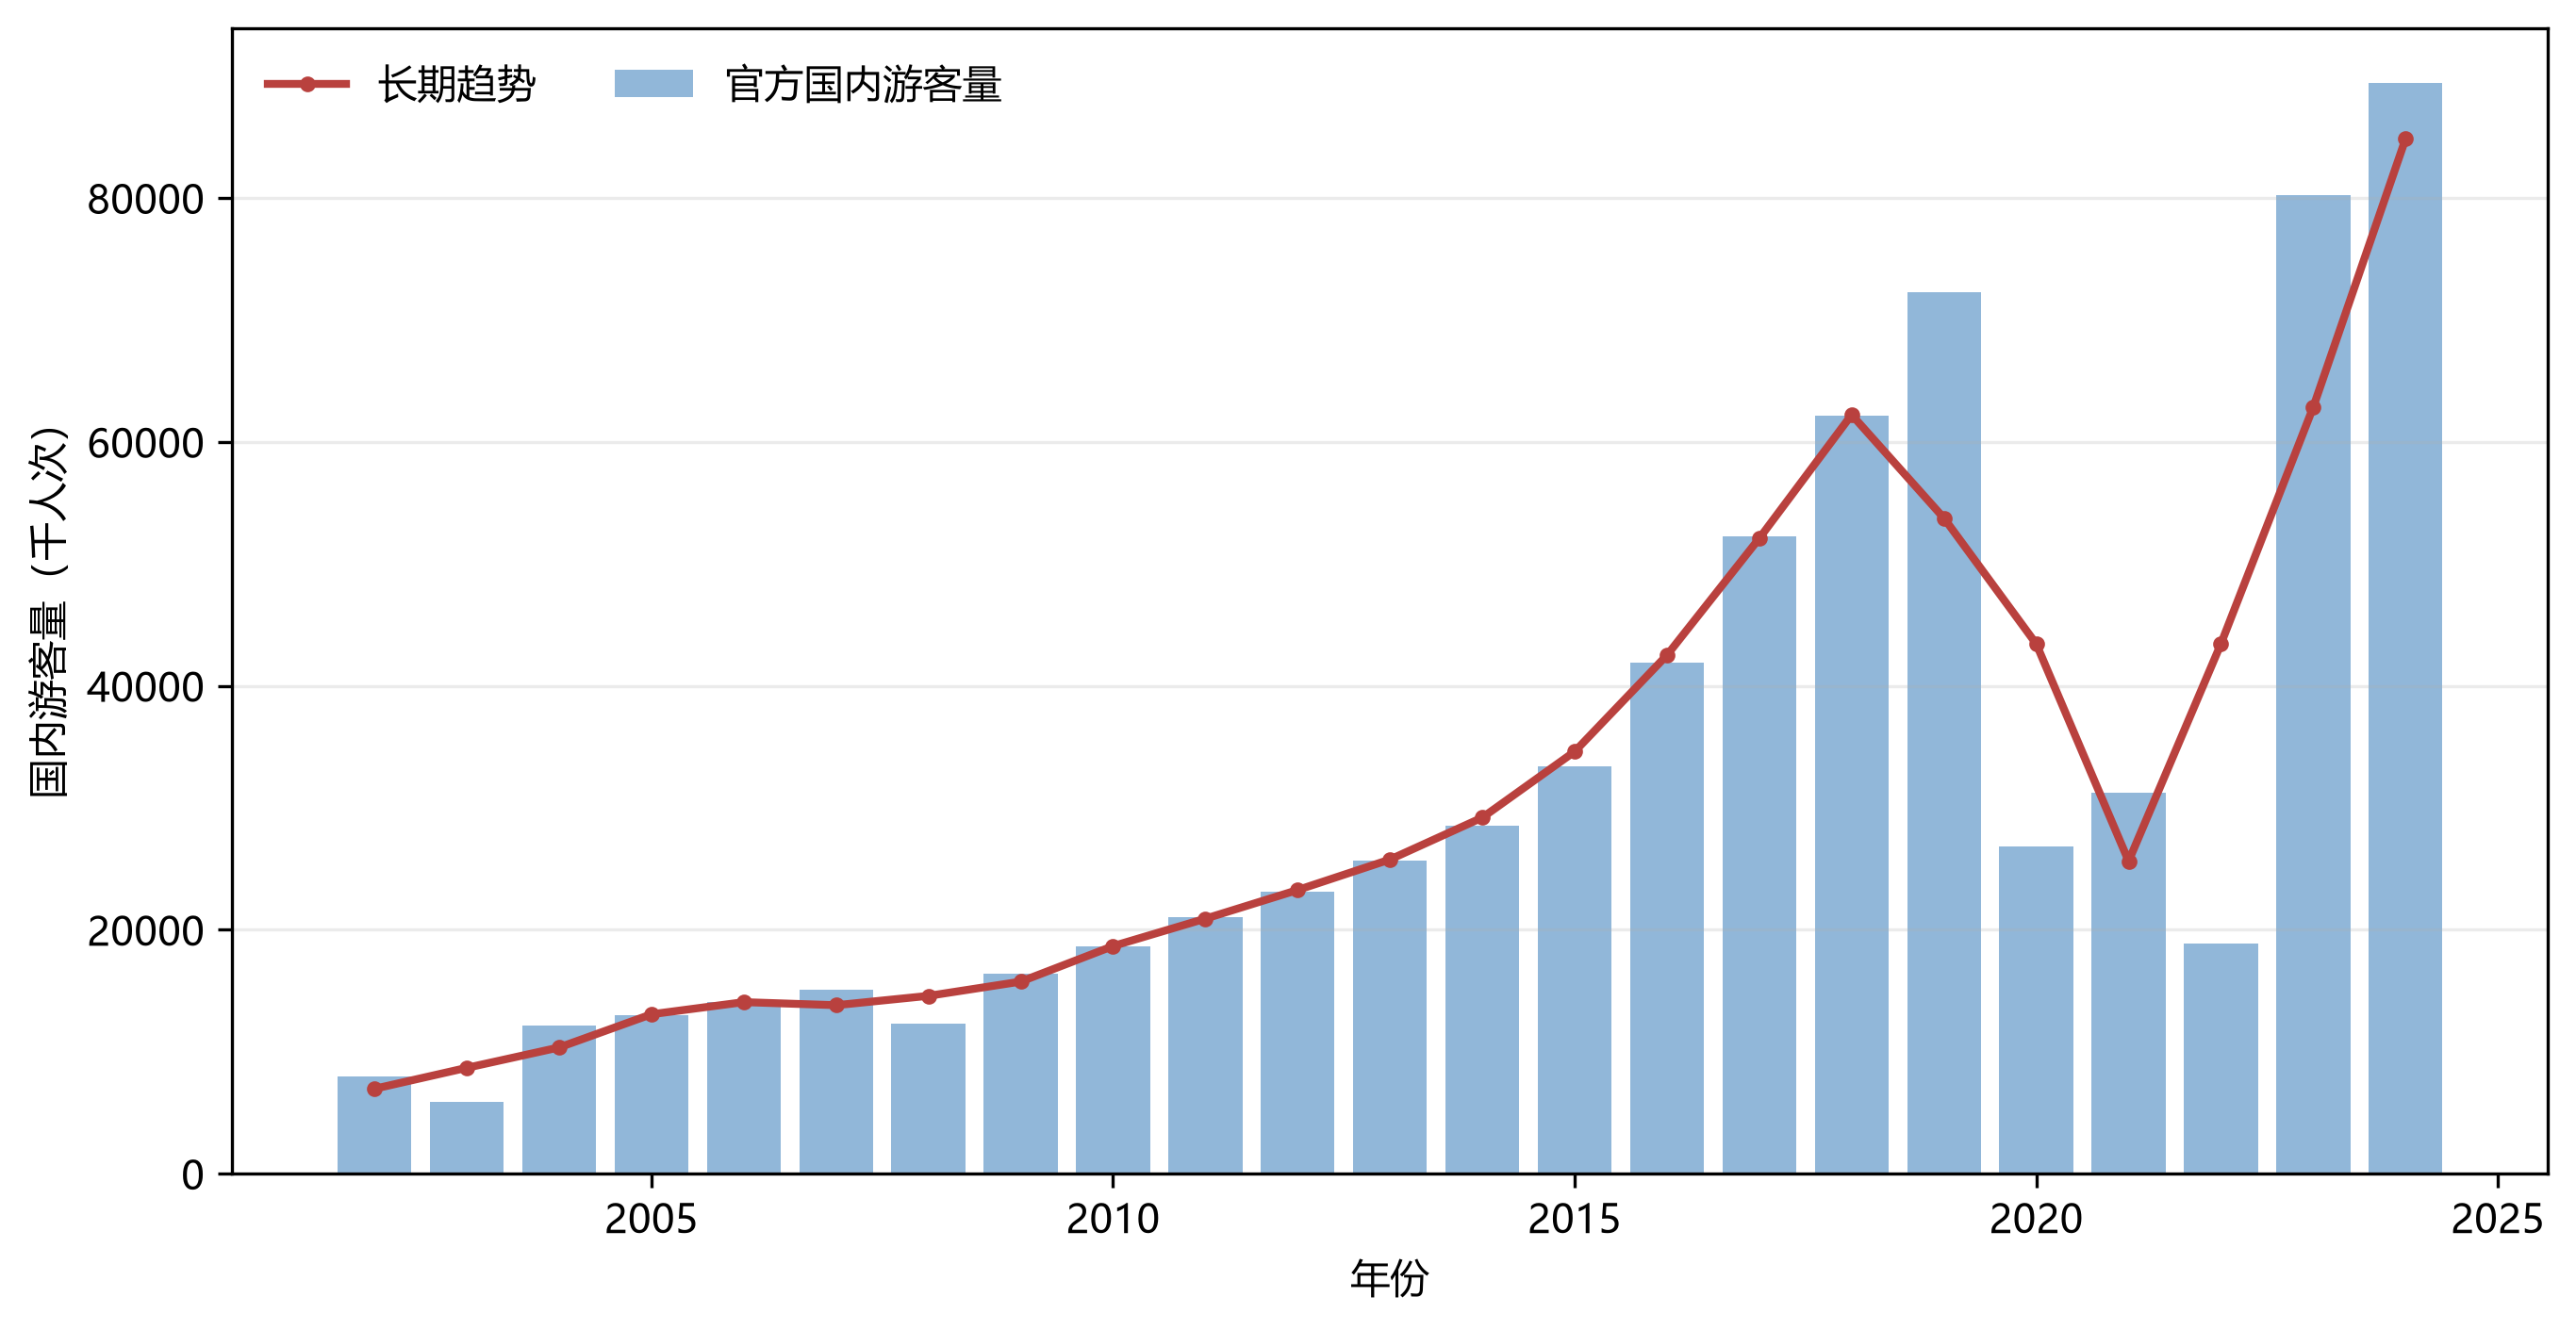
\includegraphics[width=.88\textwidth]{q1_city_annual_trend.png}
\caption{秦皇岛全市年度国内游客量及趋势}\label{fig:q1annual}
\end{figure}
\begin{figure}[H]\centering
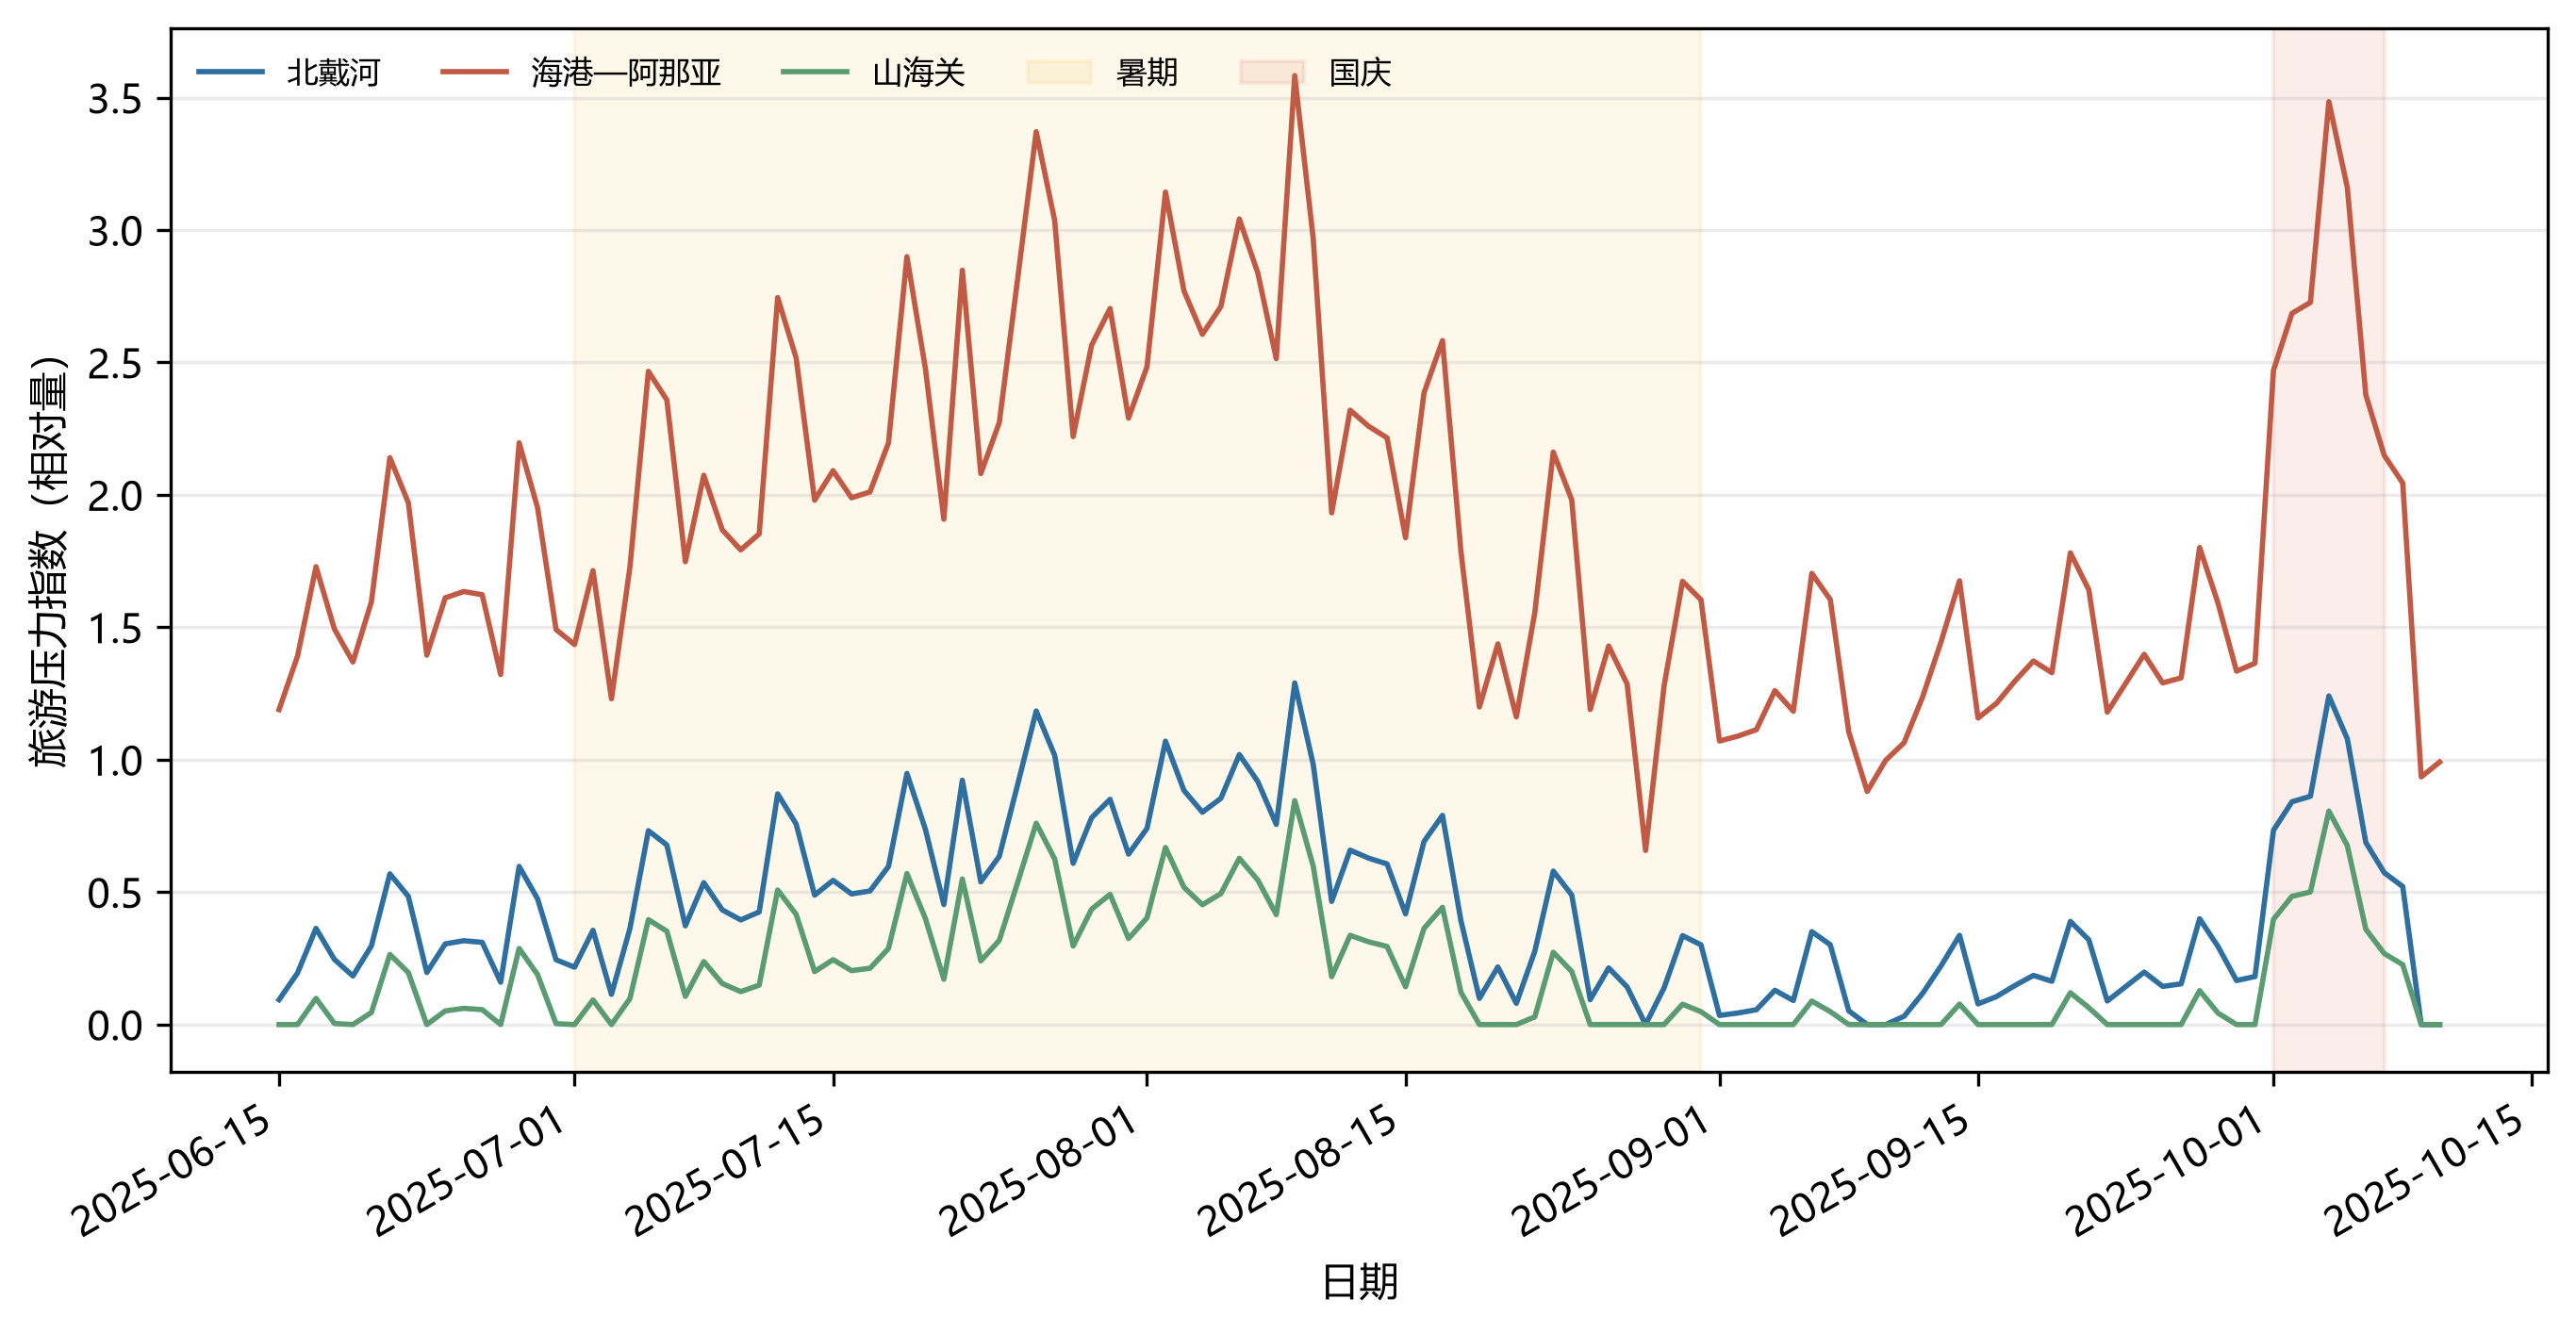
\includegraphics[width=.88\textwidth]{q1_regional_peak_pressure_2025.png}
\caption{2025 年三区日级相对旅游压力}\label{fig:q1pressure}
\end{figure}

\subsection{问题二：2026 年客流预测}
\subsubsection{年度与日级预测}
年度层比较对数趋势、上一年朴素法和近期中位增长法；日级层以 2024 年 149 条去重片区--日期观测为留出集，比较季节--日历 Ridge、动态 Ridge 和历史星期中位数。动态模型的片区搜索滞后由预预测期真实观测选择，北戴河、海港--阿那亚、山海关分别采用 1、3、2 日滞后。为避免单一全局不确定性掩盖片区差异，对三区分别实施 split-conformal 校准。

\begin{table}[H]\centering\small
\renewcommand{\arraystretch}{1.15}\setlength{\tabcolsep}{4pt}
\caption{预测模型验证结果}\label{tab:q2valid}
\begin{tabular*}{\paperTableWidth}{@{\extracolsep{\fill}}lrrr@{}}\toprule
模型 & MAE & RMSE & sMAPE(\%)\\ \midrule
年度：近期中位增长 & 11,331,292 & 24,008,187 & 24.67\\
日级：季节--日历 Ridge & 0.959 & 1.565 & 67.96\\
日级：动态 Ridge & 0.918 & 1.504 & 64.30\\
日级：历史星期中位数 & 1.160 & 2.047 & 65.90\\ \bottomrule
\end{tabular*}
\end{table}

近期中位增长法给出 2026 年全市点预测 9,971.43 万人次。动态 Ridge 的误差最低，作为日级基准；其区间覆盖率为 0.899。山海关的相对校准半径为 1.572，下界出现零截断，表示高不确定性而非零需求。

\begin{table}[H]\centering\small
\renewcommand{\arraystretch}{1.15}\setlength{\tabcolsep}{4pt}
\caption{2026 年暑期日峰值分位情景（人次）}\label{tab:q2peak}
\begin{tabular*}{\paperTableWidth}{@{\extracolsep{\fill}}lrrr@{}}\toprule
片区 & $q_{10}$ & $q_{50}$ & $q_{90}$\\ \midrule
北戴河 & 52,041 & 127,462 & 202,883\\
海港--阿那亚 & 19,230 & 58,204 & 97,179\\
山海关 & 0 & 135,474 & 348,466\\ \bottomrule
\end{tabular*}
\end{table}
\begin{figure}[H]\centering
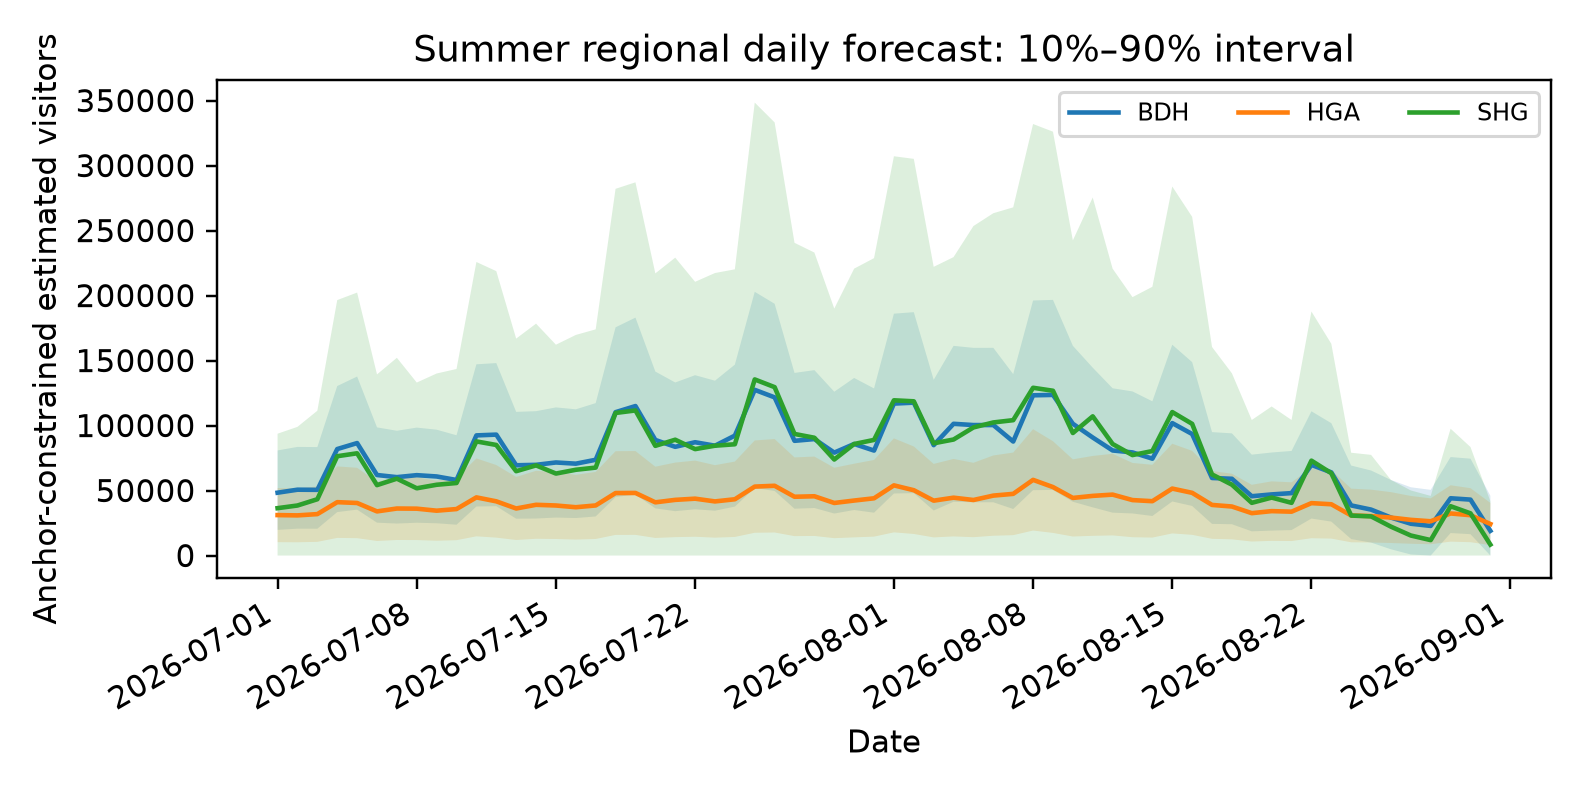
\includegraphics[width=.86\textwidth]{q2_summer_regional_daily_forecast.png}
\caption{三区 2026 年暑期日级预测及分位情景}\label{fig:q2summer}
\end{figure}

\subsection{问题三：停车、接驳与人员协同配置}
\subsubsection{决策变量、目标与约束}
对任一片区--日期情景，令 $p_d,b_d,n_d$ 分别表示可调用的临时泊位、接驳车辆和三班制人员班次；令 $u_d^P,u_d^B,u_d^N$ 表示停车、接驳和人员的服务缺口。模型以资源投入与服务不足之间的可解释折中为目标：
\begin{equation}
\min J_d=c_Pp_d+c_Bb_d+c_Nn_d+\lambda_Pu_d^P+\lambda_Bu_d^B+\lambda_Nu_d^N.
\end{equation}
其约束分别为 $P_d^{\mathrm{perm}}+p_d+u_d^P\ge P_d$、$\kappa b_dH/\tau+u_d^B\ge D_d^{\mathrm{sh}}$ 和 $N_d^{\mathrm{base}}+n_d+u_d^N\ge N_d^{\mathrm{req}}$；其中 $\kappa$ 为有效单车运力、$H/\tau$ 为高峰窗内可完成的班次。所有决策变量非负且按预设离散档位取值。已公开的节点泊位数进入 $P_d^{\mathrm{perm}}$；其余容量和运力只作为情景参数，故式(3)输出的是规划配置而非实际排班台账。

\subsubsection{需求换算与离散优化}
设 $V_d$ 为日级游客规模情景，私家车比例为 $\alpha$，平均同行人数为 $o$，高峰到达比例为 $\pi$，停留时间为 $h$，高峰窗口为 $H$，则高峰泊位需求为
\begin{equation}
P_d=\left\lceil\frac{V_d\alpha}{o}\pi\frac{h}{H}\right\rceil.
\end{equation}
接驳车辆数同时满足运输能力和最大班距约束；人员按入口、停车和驾驶三类服务在早、中、晚三班中覆盖。临时泊位、接驳车辆和人员均在 $\{0,0.2,\ldots,1\}$ 的覆盖档位中搜索，目标函数为相对运行成本与标准化服务缺口的加权和。该成本不是人民币，服务缺口也不是问卷满意度。为单独评估服务不足的经济影响，以 2024 年秦皇岛城镇居民人均可支配收入 48,700 元\cite{qhdstat} 除以 2,000 小时得到中位 VOT $24.35$ 元/(人\,h)，并取 $0.5$、$1.0$、$1.5$ 倍形成敏感性区间；它只货币化停车绕行、接驳等待和服务排队的游客时间损失，不替代资源投入目标。

北戴河 2024 年暑期旅游公交日间 15 分钟班距作为服务水平事实锚点\cite{bdhbus}；山海关火车站--景区入口的 2026 年 30 分钟班距仅作外部参照\cite{shgbus}，因范围不同不覆盖古城核心情景参数。停车占用报道未进入模型，因为其缺少与三区范围一致的连续逐时占用和泊位口径。

\begin{table}[H]\centering\small
\renewcommand{\arraystretch}{1.15}\setlength{\tabcolsep}{4pt}
\caption{Q3 关键资源需求情景}\label{tab:q3result}
\begin{tabular*}{\paperTableWidth}{@{\extracolsep{\fill}}lrrrr@{}}\toprule
片区--情景 & 峰值泊位需求 & 接驳车辆 & 人员班次 & 停车外溢日数\\ \midrule
北戴河--中位 & 9,389 & 34 & 291 & 0\\
北戴河--高压 & 27,694 & 100 & 583 & 55\\
海港--阿那亚--中位 & 3,898 & 10 & 125 & 229\\
海港--阿那亚--高压 & 12,245 & 38 & 263 & 365\\
山海关--中位 & 9,980 & 22 & 295 & 93\\
山海关--高压 & 47,566 & 137 & 966 & 249\\ \bottomrule
\end{tabular*}
\end{table}

表\ref{tab:q3result}中的外溢不是对新增停车供给的断言，而是应由外圈 P+R、预约、错峰或限流承接的管理需求。山海关 2,225 个具名古城节点泊位仅是局部硬约束，不代表全区总容量。

将数值结果转为执行动作时，停车外溢日数大于零即触发外围 P+R、预约或分时入区；接驳约束紧张时优先增加备用车辆并缩短高峰班距；人员缺口则以中班增援覆盖入口、停车和驾驶三类岗位。该映射只说明资源何时应被调用，不把模型建议表述为已经发生的运营投入。

\subsection{问题四：活动与降雨场景重优化}
\subsubsection{模型更新与反事实求解}
Q4 不另起一套资源模型，而是以 Q3 的基线日需求 $V_d$ 为起点，仅更新受扰动日的客流参数：大型活动使用 $V_d^{(c)}=V_d(1+g_d^{(c)})$ 描述预热--峰值--余波，连续降雨使用 $V_d^{(c)}=V_d(1-\rho_d^{(c)})$ 描述递进抑制；未受扰动日期保持基线值。将 $V_d^{(c)}$ 代入式(3)的需求换算和约束，得到 $x_d^{(c)}=(p_d^{(c)},b_d^{(c)},n_d^{(c)})$，并与固定基线方案 $x_d^{(0)}$ 比较最大服务缺口、资源成本和关键资源峰值。故 Q4 的差异可明确归因于场景需求更新，而非更换目标函数或评价口径。

对北戴河设置暑期大型活动的预热--峰值--余波扰动，对山海关设置连续五日降雨下的递进需求衰减。每个受扰日均与固定基线方案比较，并重新配置可变泊位、接驳和人员。

\begin{table}[H]\centering\small
\renewcommand{\arraystretch}{1.15}\setlength{\tabcolsep}{4pt}
\caption{反事实场景的重优化结果}\label{tab:q4result}
\begin{tabular*}{\paperTableWidth}{@{\extracolsep{\fill}}lccccc@{}}\toprule
场景 & \shortstack{基线最大\\服务缺口} & \shortstack{资源\\成本} & \shortstack{服务\\损失} & \shortstack{接驳车辆\\（最大）} & \shortstack{人员班次\\（最大）}\\ \midrule
活动冲击 & 0.183 & 2.200 & 0.000 & 45 & 392\\
连续降雨 & 0.259 & 2.200 & 0.099 & 22 & 295\\ \bottomrule
\end{tabular*}
\end{table}

灵敏度排序显示，接驳分担率、活动强度和私家车比例最影响最大服务缺口。因此活动前两日应根据预售和热度启动 P+R、备用接驳与中班增援；降雨情景则应收缩可变运力，但保留排水、应急引导、咨询和无障碍交通的最低班组。以中位 VOT 计，8 月 8 日活动冲击下固定基线方案的最大游客时间损失为 146,996 元，重优化后降为 0；该数为情景时间损失估计，不是运营现金流或游客赔付。图\ref{fig:q4sensitivity}给出五项情景参数对最大服务缺口的影响排序。
\begin{figure}[H]\centering
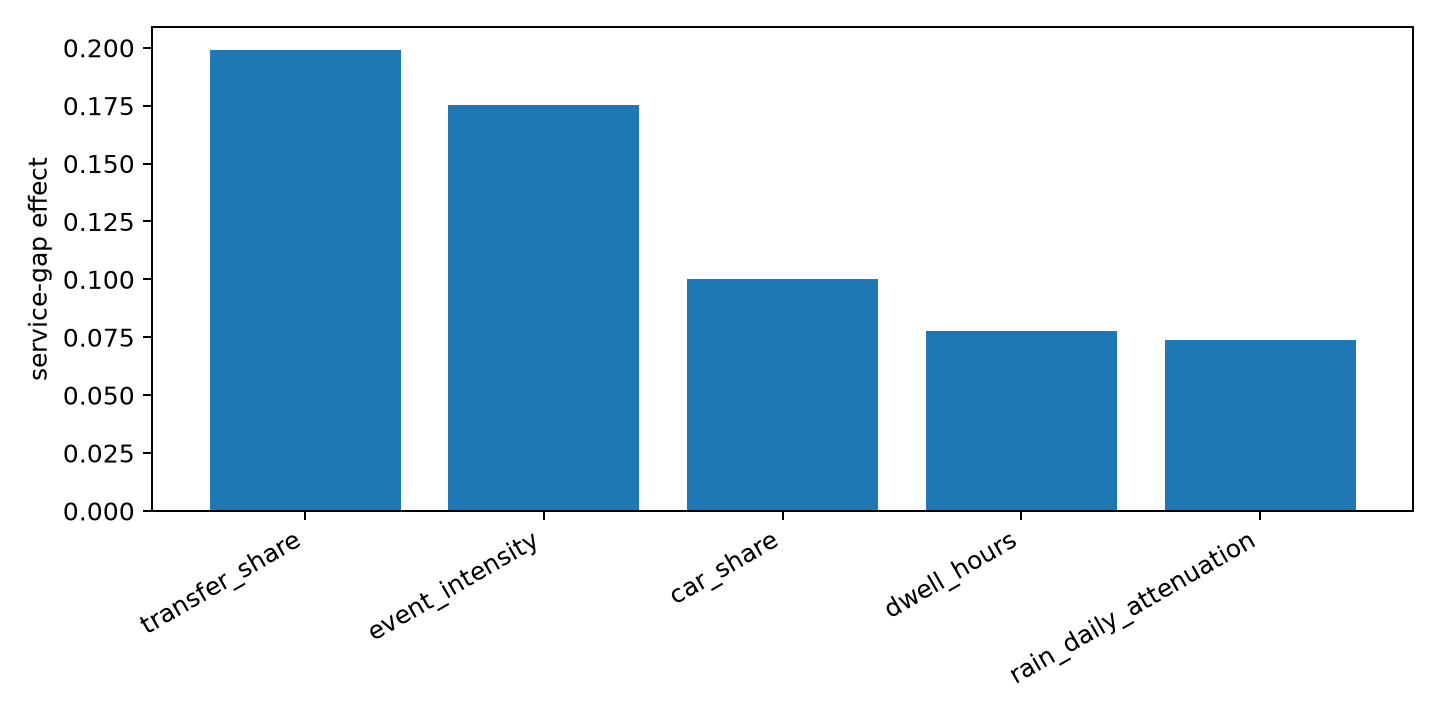
\includegraphics[width=.80\textwidth]{q4_sensitivity_ranking.png}
\caption{情景参数对最大服务缺口的影响排序}\label{fig:q4sensitivity}
\end{figure}

\section{模型分析与检验}
年度预测以留出法比较三种基准，近期中位增长法的年度 sMAPE 为 24.67\%；日级部分以 149 条去重片区--日期观测为留出集，动态 Ridge 的 MAE、RMSE 和 sMAPE 分别为 0.918、1.504 和 64.30\%，并以分片区 split-conformal 校准得到 0.899 的区间覆盖率。问题三对全部资源结果保留量纲和情景参数，问题四以反事实基线比较服务缺口，并通过五项参数扰动给出敏感性排序。因此，检验对象分别对应预测误差、区间覆盖、约束可行性和情景稳健性，而不把范围不一致的外部报道混入误差计算。

\section{模型评价、改进与推广}
本文的优点在于：将官方年度总量与片区日级相对信息分层使用；使停车、车辆、人员保持独立单位；把无法证实的运营数据显式保留为情景参数；并以重优化提供可执行的预案。局限在于缺少连续真实入园量、逐时停车占用、车辆调度与实际成本台账，因而日级游客规模和资源配置均为锚点约束估计或情景规划值。

综上，秦皇岛旅游管理应以暑期预配置、节假日动态调度和突发事件预案为主线。北戴河需优先保证旅游专线班距；海港--阿那亚需加强预约、停车和住宿的统一日台账；山海关应把古城节点饱和转化为外圈换乘和分时入城策略。获得实时闸机、停车诱导、调度和订单数据后，可将模型升级为小时级滚动优化。

\begin{thebibliography}{9}
\bibitem{qhdstat} 秦皇岛市统计局. 《秦皇岛市国民经济和社会发展统计公报》[EB/OL]. 项目原始数据登记表所列 2002--2024 年官方年度游客量来源.
\bibitem{bdhbus} 人民网河北频道. 北戴河开通旅游公交专线 2 路[EB/OL]. \url{https://he.people.com.cn/n2/2024/0705/c192235-40902683.html}.
\bibitem{shgbus} 北京日报客户端. 山海关暑期交通服务指南[EB/OL]. \url{https://peking.bjd.com.cn/content/s6a48eceee4b0e45f3fd412a0.html}.
\bibitem{shgtravel} 山海关景区. 交通指南[EB/OL]. \url{https://www.shgjq.com/jtzn/index.jhtml}.
\bibitem{aranya} 阿那亚戏剧节. Travel Information[EB/OL]. \url{https://www.aranyatheaterfestival.com/en/travel}.
\end{thebibliography}

\begin{appendices}
\section{数据与复现说明}
全部输入口径、参数边界与生成结果保存在项目的 \texttt{data}、\texttt{outputs} 和“论文写作”目录。运行 \texttt{scripts/run\_paper\_mainline.py} 可重建主线输出，运行 \texttt{pytest -q} 可执行回归测试。主线仅在 Q1--Q4 检查点均齐全时刷新 \texttt{outputs/verified\_artifacts}；若运行失败，\texttt{outputs/delivery\_status.json} 会指定已验证产物版，禁止混用失败运行的新表。公开网页来源及数据适用边界详见数据登记表与封稿核验文件。
\end{appendices}

\end{document}
